%\section{Coping with Cross Traffic}
\section{\cut{Handling }Unfavorable Conditions}\label{s:queue-ctl}

Recall from \S\ref{s:deploy} that \name can reliably shift queue build up from the bottleneck to itself when, (a) the cross-traffic is not buffer-filling, and (b) all of its component traffic shares the same bottleneck in the network.
In practice, either of these conditions may break. 
%not always hold on the real Internet, and they may change over time.
In this section, we describe how \name can re-use the same measurements from \S\ref{s:measurement} to detect when these conditions do not hold. In such cases, \name (temporarily) disables its rate limiting (falling back to status-quo performance) until favorable conditions arise again. 
%Thus, even in the worst case \name will not degrade performance (relative to the status quo without \name).
% simply degrades to status quo performance.
% Of course, in real Internet conditions, there may be scenarios where these conditions do not hold.
% In these cases, \name gracefully degrades to status quo performance. 

\subsection{Buffer-Filling Cross Traffic}
\label{s:buffer-filling}

%As \name uses a delay-minimizing congestion control algorithm to shift queue build up from the bottleneck to the \inbox.
%A well-known property of delay-minimizing congestion control algorithms is that when competing with traditional loss-based controllers, they lose throughput~\cite{copa}.

%Therefore, it is important for congestion controllers at the \inbox to detect the presence of such cross-traffic and disable the use of delay-control in these situations.
%Once the buffer-filling cross traffic leaves, the \inbox should resume delay control.

It is well known that delay-based congestion control algorithms (as \name uses) lose throughput when competing with traditional loss-based controllers~\cite{copa}. Therefore, in order to compete fairly with buffer-filling cross-traffic, \name must first detect the presence of such traffic and disable its use of a delay-based controller.  
%\paragrapha{Competing Fairly}

Prior work (Nimbus~\cite{nimbus-arxiv}) presents a method for detecting buffer-filling cross traffic, that \name employs.
\footnote{\cite{nimbus-arxiv} includes a detailed evaluation of Nimbus' accuracy of detecting buffer-filling cross traffic and speed of switching between the two modes, using both emulated and real-world experiments. Bundler's use of Nimbus does not impact its accuracy or speed of switching.}
But what exactly should the \inbox do when it detects this condition?
A naive approach might replace the delay-based control at \name with a loss-based buffer-filling congestion control such as Cubic. 
However, with this approach, \name must measure the number of flows in a bundle, and should compete as aggressively in proportion to achieve an aggregate throughput equivalent to status quo~\cite{multcp}. On high-performance datapaths, it may be difficult to measure this number~\cite{heavy-hitters}.

We propose a simpler solution.
Since bundles comprise of traditional end-host connections, with their own congestion controllers, \name can simply \emph{let the traffic pass}, \ie increase the pacing rate at the \inbox to stop controlling queues. Then, the end-host congestion control loop will naturally compete fairly with the aggressive cross traffic, just as traffic in the Internet does today.
%Copa is not compatible with this approach because its TCP-compatible mode is designed for the context of a single connection. Therefore, we must use Nimbus~\cite{nimbus} for cross traffic detection.

%\paragrapha{Active Probing}
This brings us to the next natural question: How can the \inbox know it is safe to resume delay-control (and scheduling) after disabling it?
%It is important to distinguish between \emph{self-inflicted} queueing delay and queueing delay due to cross traffic.
%When the queueing delay is purely self-inflicted, it is safe to resume control over the queues at the \inbox.
One approach is to send passive probes along the network to detect the presence/absence of queuing. However, such passive measurements cannot distinguish between the self-inflicted queuing due to \name's traffic and the queuing due to cross-traffic. If the bottleneck queue is entirely self-inflicted, it is safe (and desirable) to resume delay-control and scheduling.
%Passive probing is insufficient to determine this state, since passive measurements of the bottleneck will be identical in the case of self-inflicted queueing and queueing driven by cross traffic.
Therefore, it is important to \emph{actively probe}, that is, change the rate of bundled traffic and observe the response of the cross traffic. 
This is what the Nimbus mechanism does.
At a high level,
Nimbus sinusoidally varies the sending rate $r(t) = A sin(\frac{4\pi{}t}{T})$ during the up-pulse, where $A$ is the pulse amplitude (set to one-fourth of the estimated bottleneck bandwidth) and $T$ is the pulse duration, and measures the cross traffic's response in the frequency domain.
The \inbox can use the Nimbus algorithm to detect when to relinquish control over the queue by interposing this sending pattern over the delay-controller's rate decisions.
However, if the \inbox entirely drains its queues into the network, it will no longer be possible for Nimbus to overlay pulses onto the traffic pattern, and it will be unable to determine the nature of the cross traffic.
Practically, this would mean that once \inbox switches to compete with cross traffic, it would never gain the information necessary to switch back.

Instead, to support active probing while also letting the traffic pass, the \inbox must maintain some queueing.
How many packets should this be? The \inbox should be able to generate enough packets for a Nimbus up-pulse, \ie the area under the up-pulse curve: 
$A \int_0^{\frac{T}{4}} \sin(\frac{4\pi{}t}{T}) dt = \frac{AT}{2\pi}$.
From Nimbus, we use $T = 0.2$ seconds and $A$ is as above, one-fourth the bottleneck bandwidth. By Little's law, we can calculate the amount of extra queueing: $\frac{T}{8\pi}$, or $8$ms.
We thus configure the \inbox to hold back $10$ms of queueing for active probing; the additional queueing is a cushion against input variance.
Note that this extra queueing is in addition to queueing in the network. As a result, the end-to-end Cubic connections will see mild RTT inflation.
In \S\ref{s:robust:cross} we show that this effect is not large; \name still achieves performance comparable to the status quo.

How should we achieve this target queueing delay? 
This problem is similar to the role of the PIE AQM mechanism~\cite{pie}, which also seeks to maintain a queueing delay target.
Correspondingly, we design a PI controller at the \inbox as part of the fairness control module. 
It overlays a rate $r$ corresponding to $\dot{r}(t) = \alpha (q - q_T) + \beta (\dot{q})$, where $q$ is the queue size and $q_T$ is the target queue size computed above.
We pick $\alpha = 10$ and $\beta = 10$ by solving for a convergence time of one RTT (Appendix~\ref{app:derive-ab}).
% as per \S\ref{s:qctl:pi}.

\begin{Appendix}
\section{Queue Controller Stability}\label{app:derive-ab}

We control the queues with the update function 
\begin{equation} 
    \dot{r}(t) = \alpha (q - q_T) + \beta (\dot{q})
\end{equation}

How should we set $\alpha$ and $\beta$? This decision is related to the size of the Nimbus pulse. 
If the queue controller is too aggressive (\ie it reacts quickly to maintain the queue target), it will nullify the Nimbus pulse with its overlaid rate control.
If it is too timid, it will not be able to effectively control the queues.

Therefore, we want the target queue length to be $A \sin(\frac{2\pi{}t}{T})$. 
We can write how the queue length varies with time as (where $\mu$ is the link bandwidth):
\begin{equation} 
    \dot{q}(t) = \mu - r(t) - A \sin(\frac{2\pi{}t}{T})
\end{equation}

\noindent Thus, 

\begin{equation}
    \ddot{q}(t) = - \dot{r}(t) - A \frac{2\pi{}t}{T} \cos(\frac{2\pi{}t}{T})
\end{equation}

\noindent Combining with the rate update rule:

\begin{equation}
    \ddot{q}(t) - \beta \dot{q}(t) + \alpha (q(t) - q_T) = A \frac{2\pi{}t}{T} \cos(\frac{2\pi{}t}{T})
\end{equation}

\noindent Substituting the pulse parameters from Nimbus and using $y(t) = q(t) - q_T$, we write a second-order ordinary differential equation (ODE) with sinusoidal input:

\begin{equation}
    \ddot{y}(t) - \beta \dot{y}(t) + \alpha y(t) = 10\pi{}A \cos(10\pi{}t)
\end{equation}

    \noindent This has the standard-form solution:

\begin{equation}
    y(t) = c_1 e^{r_1 t} + c_2 e^{r_2 t} + \frac{10\pi{}A}{|p(10\pi{}i)|} \cos(10\pi{}i - \phi)
\end{equation}
        
where $p$ is the characteristic polynomial and $r_1, r_2$ are its roots;
\ie, 
\begin{equation}
r_1 = \frac{-\beta + \sqrt{\beta^2 - 4\alpha}}{2}, r_2 = \frac{-\beta - \sqrt{\beta^2 - 4\alpha}}{2}
\end{equation}

\noindent We want: (1) the $r_1$, $r_2$ to be large, so the queue converges quickly, and (2) the pulse amplitude to be approximately the Nimbus pulse amplitude, so:

\begin{equation}
\frac{10\pi{}A}{|p(10\pi{}i)|} \approx \frac{A}{5\pi}
\end{equation}

$\alpha = 10, \beta = 10$ satisfy these constraints.
\end{Appendix}

\subsection{Imbalanced Multipathing}\label{s:queue-ctl:ecmp}
Since a \bundle contains many component connections, a load balancer may send them along different paths. If the load along different paths is well-balanced, \name will accurately treat a load-balanced bottleneck link as a single link with the aggregate rate of each sub-link. However, when the load along different paths is imbalanced, the series of measurements at the \name will be a random sampling of the different paths, which would confuse the delay-control algorithm and cause it to perform poorly. Fortunately, such cases are straight-forward to detect with our measurement technique. 
More specifically, load imbalance will result in many epoch measure packets arriving out-of-order at the \outbox (whenever epoch packet $i$ happens to traverse a path with a larger delay than epoch packet $i+1$), and consequently, out-of-order ``congestion ACKs'' at the \inbox.  Figure~\ref{fig:queue-ctl:ecmp:motivation} shows this effect for an emulated imbalance scenario. Therefore, we use the fraction of epoch measurement packets that arrive out-of-order as an indicator of load imbalance due to multipathing. 
If this number is small, the links are roughly balanced and \name will operate correctly.
If it is large, it indicates load imbalance, in which case \name's rate-control would work incorrectly. 
%While we believe that it is possible to design a rate controller that distinguishes RTT samples from different paths, and computes appropriate aggregate rates, we leave this for future research, and instead adopt a simpler
%the delay controller will make erratic adjustments as it briefly observes high RTTs, and may lose throughput as a result.
Therefore, if the reordering level is above 5\%, we disable rate control and revert to status quo performance. We evaluate this approach (and justify our chosen threshold) in \S\ref{s:eval:ecmp}.
%In this case, the measurement sub-system (\S\ref{s:measurement}) would report erratic measurements corresponding in turn to each of the possible paths.
% To see why, consider that \name's epoch-based rate measurements do not distinguish the path the packets take, and instead consider only the number of packets sent and received in an epoch.
% Thus, \name will accurately measure a load-balanced bottleneck link as a single link with the aggregate rate of each sub-link.
% However, for RTT measurements, the link with the lowest RTT will be over-sampled because the first epoch feedback packet to arrive will be from this link.
% So, \name will not detect building queues in other links.
% In most cases, this is not fatal: the delay controller might yield too much queue to the bottleneck, causing \name to miss out on performance improvements.
% We leave the design of a delay controller that does not over-react to conflicting measurements, and thus further optimizes traffic-control ability, to future work.

%In extreme cases, there may be persistent imbalance in the level of queueing. 

\begin{figure}
    \centering
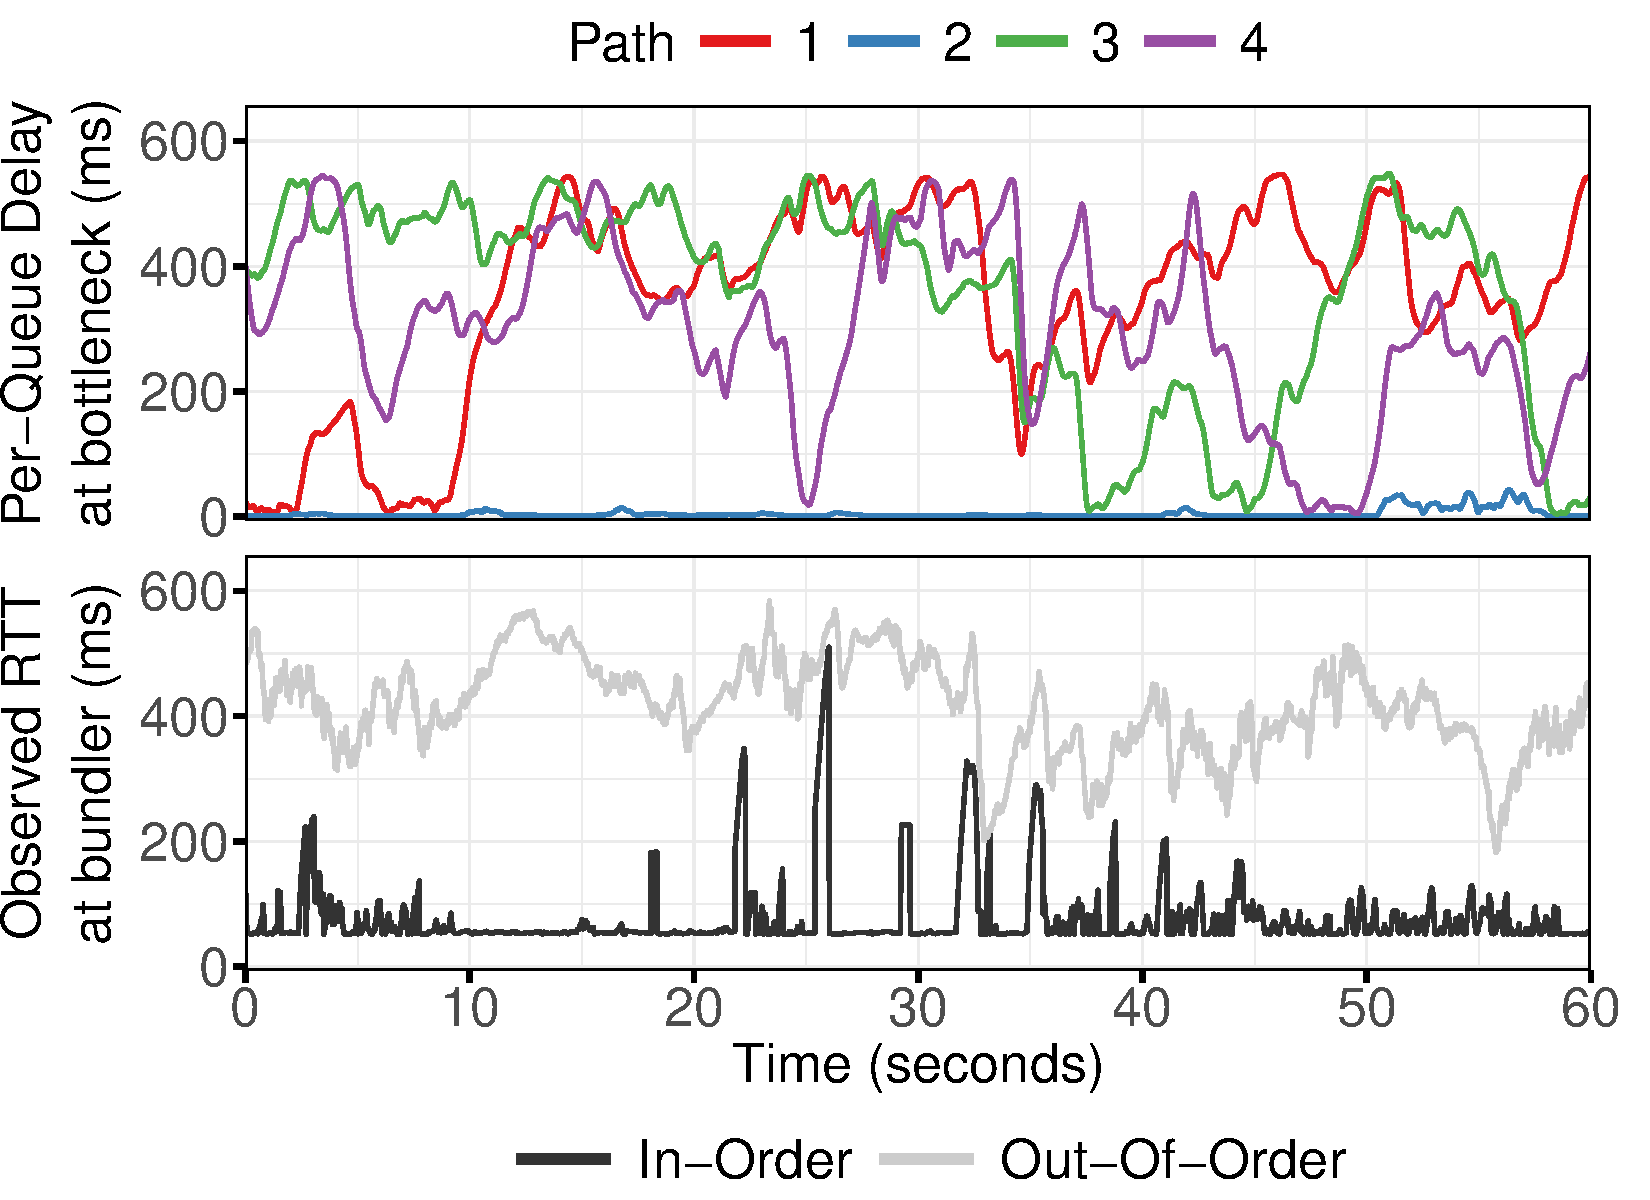
\includegraphics[width=\maxwidth]{figure/ecmp_delay.pdf} 
\vspace{2pt}
\caption{(Top) True delay for all packets of \name's component flows based on which of 4 load-balanced paths they traversed (unknown to \name). (Bottom) Delay measurements observed by Bundler, colored based on whether they were derived from an in-order or out-of-order epoch packet. Bundler's measurements cannot distinguish how many paths there are, but the relative number of out-of-order measurements is enough to clearly indicate the presence of multiple RTT-imbalanced paths.}
\label{fig:queue-ctl:ecmp:motivation}
\end{figure}

\cut{
\begin{outline}

\1 Since a \bundle contains many component connections, a load balancer may send them along different paths.
\1 In this case, a naive implementation of the measurement sub-system would report erratic measurements.
    \2 The delay controller would correspondingly set suboptimal rates.
    \2 In many cases, this is ok; the delay controller will yield too much queue to the bottleneck, but there will still be a partial queue at the \inbox to schedule.
    \2 We evaluate this system in~\S\ref{s:eval:realworld} and find that \name can cope with multipath in real scenarios.
\1 In extreme cases, which we can detect by looking at the amount of reordering, we can disable the delay controller and revert to status quo performance. We evaluate this in~\S\ref{s:eval:ecmp}.
\end{outline}

Alternative outline if we want to get into more detail:
\begin{outline}
\1 In reality, different flows traveling between the same inbox and outbox may traverse different paths across the internet.
\1 What matters is how different (heterogenous?) these paths are (because if they're all exactly the same it'd be equivalent to one link from the perspective of rtt and recv\_rate).
\1 First, consider the possibility that packets take a truly different path (defined as sequence of distinct routers) across the internet between inbox and outbox. Our measurements in X show this does not often happen in practice.
\1 Of course, even if they follow the same sequence of routers, these routers may be connected by multiple physical links which are load balanced via ECMP.
\1 In this case, the ECMP’d links act the same as one with the sum of their capacity, but the issue is different packets may experience different latencies depending on the load of the link they happen to get hashed to.
\1 In both this case, and the case where they take totally different paths, the symptoms are similar -- the measurement sub-system would report erratic measurements that the CC scheme is unprepared to handle. It turns out, although we may not be able to distinguish which case it is, we can reliably detect this symptom (briefly explain re-ordering heuristic), and in these cases we can disable bundler to ensure we revert back to status quo performance. We evaluate this in Y.
\1 Thus, even in the worst case, bundler does at least as good as status quo. But when there is opportunity to do so, it achieves benefits.
We believe it would be possible to modify our congestion control scheme to incorporate out of order measurements, which may increase the set of scenarios in which Bundler can provide benefits, but we leave this as an area of future work.
\end{outline}
}
